% =====================================================================
%  CIS 112 -- Week 1: Version Control Systems (Git)
%  LaTeX Beamer conversion of cis112-w01-VCS-20250928.pptx
%
%  Compile with:  pdflatex cis112-w01-VCS.tex   (run twice)
%  Images are expected in ./images/
% =====================================================================
\documentclass[aspectratio=169,11pt,t]{beamer}

\usepackage[utf8]{inputenc}
\usepackage[T1]{fontenc}
\usepackage[scaled=0.92]{helvet}
\usepackage{courier}
\usepackage{microtype}
\DisableLigatures[-]{encoding=T1,family=tt*}  % keep -- as two hyphens in commands
\renewcommand{\familydefault}{\sfdefault}
\usepackage{graphicx}
\usepackage{array}
\usepackage{xcolor}
\usepackage{listings}
\usepackage{tikz}
\usetikzlibrary{arrows.meta,positioning}
\graphicspath{{images/}}

% ---------------------------------------------------------------------
%  Colours (taken from the original deck)
% ---------------------------------------------------------------------
\definecolor{accent}{HTML}{FFC000}     % titles and highlighted terms
\definecolor{cmdcol}{HTML}{D99A00}     % git commands (a little darker for legibility)
\definecolor{bulletblue}{HTML}{000080}
\definecolor{linkcol}{HTML}{467886}
\definecolor{vnode}{HTML}{1F5F8B}
\definecolor{gitteal}{HTML}{1AAE98}
\definecolor{gitnavy}{HTML}{0B1540}
\definecolor{gitbrown}{HTML}{5E3D1E}
\definecolor{wdgreen}{HTML}{B3D6B0}
\definecolor{idxorange}{HTML}{FFB687}
\definecolor{repoblue}{HTML}{8AB4EA}

% ---------------------------------------------------------------------
%  Beamer look
% ---------------------------------------------------------------------
\setbeamertemplate{navigation symbols}{}
\setbeamercolor{normal text}{fg=black}
\setbeamercolor{structure}{fg=bulletblue}
\setbeamercolor{frametitle}{fg=accent}
\setbeamerfont{frametitle}{size=\LARGE}
\setbeamertemplate{frametitle}{\vskip4mm\usebeamerfont{frametitle}\insertframetitle\par\vskip1mm}
\setbeamertemplate{itemize item}{\color{bulletblue}\small$\blacksquare$}
\setbeamertemplate{itemize subitem}{\color{gray}\scriptsize$\square$}
\setbeamertemplate{itemize subsubitem}{\color{bulletblue}\tiny$\blacksquare$}
\setbeamerfont{itemize/enumerate body}{size=\normalsize}
\setbeamerfont{itemize/enumerate subbody}{size=\small}
\setbeamerfont{itemize/enumerate subsubbody}{size=\footnotesize}
\setbeamersize{text margin left=9mm,text margin right=9mm}
\setbeamertemplate{footline}{%
  \color{gray}\tiny
  \hbox to\paperwidth{\hfill Git\hfill\llap{\insertframenumber\hspace*{8mm}}}\vskip2.5mm}

% ---------------------------------------------------------------------
%  Helpers
% ---------------------------------------------------------------------
\newcommand{\hl}[1]{\textcolor{accent}{#1}}              % highlighted term
\newcommand{\cmd}[1]{\textcolor{cmdcol}{\texttt{#1}}}    % git command
\newcommand{\ph}[1]{\textit{#1}}                         % placeholder argument
\newcommand{\link}[1]{\textcolor{linkcol}{\underline{\texttt{#1}}}}
% centred orange section divider
\newcommand{\dividerslide}[1]{%
  \begin{frame}[c]
    \centering{\LARGE\color{accent}#1\par}
  \end{frame}}

% version stacks (v5 -> v6 -> v7) used on the motivation slides
\tikzset{
  ver/.style={circle,draw=vnode,thick,minimum size=6mm,inner sep=0pt,font=\scriptsize},
  vernew/.style={ver,draw=accent,dashed,text=accent,rectangle,rounded corners=1pt},
  varr/.style={-{Latex[length=1.6mm]},vnode,thick},
  commit/.style={circle,draw=black,thick,minimum size=6mm,inner sep=0pt},
  cmain/.style={commit,fill=gitteal},
  cfeat/.style={commit,fill=gitnavy},
  cxyz/.style={commit,fill=gitbrown},
  ref/.style={font=\rmfamily\bfseries\scriptsize},
  refarr/.style={-{Straight Barb[length=1.4mm,open]}},
}
\newcommand{\stack}[4]{% x, top label, bottom caption, style of top node
  \node[ver] (#1a) at (#1,0) {v5};
  \node[ver] (#1b) at (#1,1) {v6};
  \node[#4] (#1c) at (#1,2) {#2};
  \draw[varr] (#1a) -- (#1b);
  \draw[varr] (#1b) -- (#1c);
  \node[font=\scriptsize] at (#1,-0.65) {#3};}
\newcommand{\teamdiagram}{%
  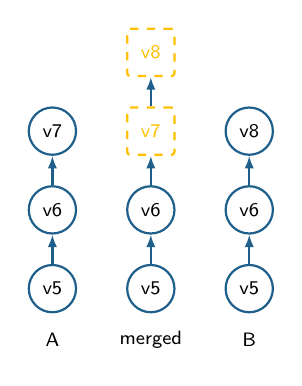
\begin{tikzpicture}[x=1.25cm]
    \stack{0}{v7}{A}{ver}
    \stack{2}{v8}{B}{ver}
    \node[ver] (ma) at (1,0) {v5};
    \node[ver] (mb) at (1,1) {v6};
    \node[vernew] (mc) at (1,2) {v7};
    \node[vernew] (md) at (1,3) {v8};
    \draw[varr] (ma) -- (mb);
    \draw[varr] (mb) -- (mc);
    \draw[varr] (mc) -- (md);
    \node[font=\scriptsize] at (1,-0.65) {merged};
  \end{tikzpicture}}

\lstset{basicstyle=\ttfamily\footnotesize,columns=fullflexible,keepspaces=true,
        upquote=true,showstringspaces=false}

\title{Version Control Systems (Git)}
\date{}

\begin{document}

% =====================================================================
%  1  Title
% =====================================================================
\begin{frame}[c,plain]
  \centering
  {\large cis112\par}
  \vskip1mm
  {\fontsize{28}{32}\selectfont\color{accent}Version Control\\ Systems (Git)\par}
  \vskip10mm
  BBBF\\
  Yeditepe University\\[5mm]
  {\scriptsize V2025-02-17}
\end{frame}

% =====================================================================
%  2  Agenda
% =====================================================================
\begin{frame}{Agenda}
  \vskip4mm
  \begin{itemize}
    \item Why use Version (Source) Control Systems?
    \item What are Git and GitHub?
    \item Basic Git Commands
  \end{itemize}
\end{frame}

% =====================================================================
%  3--4  Motivation
% =====================================================================
\section{Motivation}
\dividerslide{Motivation}
\dividerslide{Motivation\\ for the\\ Single Programmer}

% =====================================================================
%  5  Why version control?
% =====================================================================
\begin{frame}{Why version control?}
  \begin{columns}[T]
    \begin{column}{0.72\textwidth}
      \vskip4mm
      \begin{itemize}
        \item Scenario 1:
          \begin{itemize}
            \item Your program is working
            \item You change ``just one thing''
            \item Your program breaks
            \item You change it back
            \item Your program is still broken--\emph{why?}
          \end{itemize}
        \vskip3mm
        \item Has this ever happened to you?
      \end{itemize}
    \end{column}
    \begin{column}{0.24\textwidth}
      \vskip14mm
      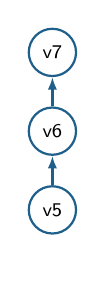
\begin{tikzpicture}\stack{0}{v7}{}{ver}\end{tikzpicture}
    \end{column}
  \end{columns}
\end{frame}

% =====================================================================
%  6  Why version control? (part 2)
% =====================================================================
\begin{frame}{Why version control? (part 2)}
  \begin{columns}[T]
    \begin{column}{0.72\textwidth}
      \vskip2mm
      \begin{itemize}
        \item Your program worked well enough yesterday
        \item You made a lot of improvements last night\ldots
          \begin{itemize}
            \item \ldots but you haven't gotten them to work yet
              \begin{itemize}
                \item You need to turn in your program \emph{now}
              \end{itemize}
          \end{itemize}
        \vskip3mm
        \item Has this ever happened to you?
      \end{itemize}
    \end{column}
    \begin{column}{0.24\textwidth}
      \vskip14mm
      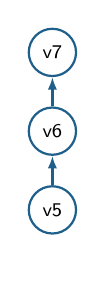
\begin{tikzpicture}\stack{0}{v7}{}{ver}\end{tikzpicture}
    \end{column}
  \end{columns}
\end{frame}

% =====================================================================
%  7  Motivation for a Team
% =====================================================================
\dividerslide{Motivation\\ for a\\ Team of Programmers}

% =====================================================================
%  8  Version control for teams
% =====================================================================
\begin{frame}{Version control for teams}
  \begin{columns}[T]
    \begin{column}{0.64\textwidth}
      \vskip4mm
      \begin{itemize}
        \item Scenario:
          \begin{itemize}
            \item You change one part of a program--it works
            \item Your co-worker changes another part--it works
            \item You put them together--it doesn't work
            \item Some change in one part must have broken something in the other part
            \item What were all the changes?
          \end{itemize}
      \end{itemize}
    \end{column}
    \begin{column}{0.34\textwidth}
      \vskip2mm
      \centering\teamdiagram
    \end{column}
  \end{columns}
\end{frame}

% =====================================================================
%  9  Teams (part 2)
% =====================================================================
\begin{frame}{Teams (part 2)}
  \begin{columns}[T]
    \begin{column}{0.64\textwidth}
      \vskip6mm
      \begin{itemize}
        \item Scenario:
          \begin{itemize}
            \item You make a number of improvements to a class
            \item Your co-worker makes a number of \emph{different} improvements to the \emph{same} class
          \end{itemize}
        \vskip2mm
        \item How can you merge these changes?
      \end{itemize}
    \end{column}
    \begin{column}{0.34\textwidth}
      \vskip2mm
      \centering\teamdiagram
    \end{column}
  \end{columns}
\end{frame}

% =====================================================================
%  10  Version Control Systems
% =====================================================================
\section{Version Control Systems}
\dividerslide{Version Control Systems}

% =====================================================================
%  11  Version control systems
% =====================================================================
\begin{frame}{Version control systems}
  \vskip3mm
  \begin{itemize}
    \item A \hl{version control system} (often called a \hl{source code control system}) does these things:
      \begin{itemize}
        \item Keeps multiple versions (older and newer) of everything (not just source code)
        \item Requests \hl{comments} regarding every change
        \item Allows ``\hl{check in}'' and ``\hl{check out}'' of files so you know which files someone else is working on
        \item Displays \hl{differences} between versions
      \end{itemize}
  \end{itemize}
\end{frame}

% =====================================================================
%  12  Benefits of version control
% =====================================================================
\begin{frame}{Benefits of version control}
  \vskip3mm
  \begin{itemize}
    \item For working \hl{by yourself}:
      \begin{itemize}
        \item Gives you a ``time machine'' for going back to earlier versions
        \item Gives you great support for different versions (standalone, web app, etc.) of the same basic project
      \end{itemize}
    \item For working \hl{with others}:
      \begin{itemize}
        \item Greatly simplifies concurrent work, merging changes
      \end{itemize}
  \end{itemize}
\end{frame}

% =====================================================================
%  13  Git and GitHub
% =====================================================================
\section{Git and GitHub}
\dividerslide{Git and GitHub}

% =====================================================================
%  14  What are Git and GitHub?
% =====================================================================
\begin{frame}{What are Git and GitHub?}
  \vskip3mm
  \begin{itemize}
    \item \hl{Git} is a \hl{free} and \hl{open source}, \hl{distributed} \textbf{version control system}
          designed to handle everything from small to very large projects with speed and efficiency.
    \item \hl{GitHub} is a \textbf{web-based} Git repository \textbf{\hl{hosting service}}, which offers
          all of the distributed revision control and \hl{source code management} (\hl{SCM})
          functionality of Git as well as adding its own features. GitHub is also free (as in free beer).
  \end{itemize}
\end{frame}

% =====================================================================
%  15  GitHub
% =====================================================================
\begin{frame}{GitHub}
  \vskip3mm
  \begin{itemize}
    \item \link{https://github.com/}
    \item When looking for a software developer position, host substantial projects you have
          developed on GitHub and give a link in your resume.
  \end{itemize}
\end{frame}

% =====================================================================
%  16  About Git
% =====================================================================
\begin{frame}{About Git}
  \begin{columns}[T]
    \begin{column}{0.66\textwidth}
      \small
      \begin{itemize}
        \item Created by \hl{Linus Torvalds}, who is the creator of \hl{Linux kernel}, in 2005
          \begin{itemize}
            \item Came out of Linux development community
            \item Designed to do version control on Linux kernel
          \end{itemize}
        \item Goals of Git:
          \begin{itemize}
            \item \hl{Speed}
            \item Support for \hl{non-linear development} (thousands of parallel branches)
            \item Fully \hl{distributed}
            \item Able to handle large projects efficiently
          \end{itemize}
        \vskip2mm
        \item[] (A ``git'' is a cranky old man. Linus meant himself.)
      \end{itemize}
    \end{column}
    \begin{column}{0.3\textwidth}
      \centering
      
\includegraphics[width=0.62\linewidth]{git-logo.png}\\[5mm]
      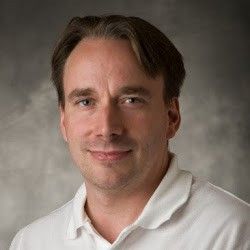
\includegraphics[width=0.75\linewidth]{linus-torvalds.jpeg}
    \end{column}
  \end{columns}
\end{frame}

% =====================================================================
%  17  Centralized VCS
% =====================================================================
\begin{frame}{Centralized VCS}
  \begin{columns}[T]
    \begin{column}{0.56\textwidth}
      \small
      \begin{itemize}
        \item In \hl{Subversion}, \hl{CVS}, \hl{Perforce}, etc., a central server repository (repo)
              holds the ``official copy'' of the code
          \begin{itemize}
            \item the server maintains the sole version history of the repo
          \end{itemize}
        \item You make ``checkouts'' of it to your local copy
          \begin{itemize}
            \item you make local modifications
            \item your changes are not versioned
          \end{itemize}
        \item When you're done, you ``check in'' back to the server
          \begin{itemize}
            \item your checkin increments the repo's version
          \end{itemize}
      \end{itemize}
    \end{column}
    \begin{column}{0.42\textwidth}
      \vskip12mm
      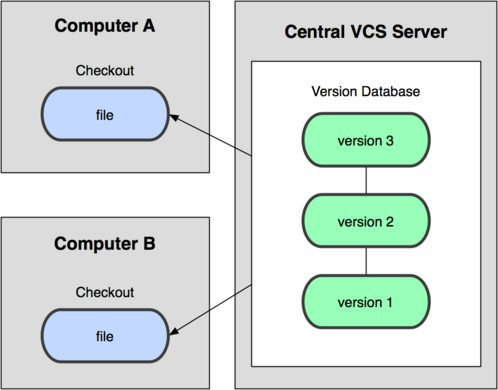
\includegraphics[width=\linewidth]{centralized-vcs.jpeg}
    \end{column}
  \end{columns}
\end{frame}

% =====================================================================
%  18  Distributed VCS (Git)
% =====================================================================
\begin{frame}{Distributed VCS (Git)}
  \begin{columns}[T]
    \begin{column}{0.6\textwidth}
      \small
      \begin{itemize}
        \item In \hl{git}, \hl{mercurial}, etc., you don't ``checkout'' from a central repo
          \begin{itemize}
            \item you ``\hl{clone}'' it and ``\hl{pull}'' changes from it
          \end{itemize}
        \item Your local repo is a \hl{complete copy} of everything on the remote server
          \begin{itemize}
            \item yours is ``just as good'' as theirs
          \end{itemize}
        \item Many operations are local:
          \begin{itemize}
            \item \hl{check in/out} from local repo
            \item \hl{commit} changes to local repo
            \item local repo keeps version history
          \end{itemize}
        \item When you're ready, you can ``\hl{push}'' changes back to server
      \end{itemize}
    \end{column}
    \begin{column}{0.36\textwidth}
      \vskip4mm
      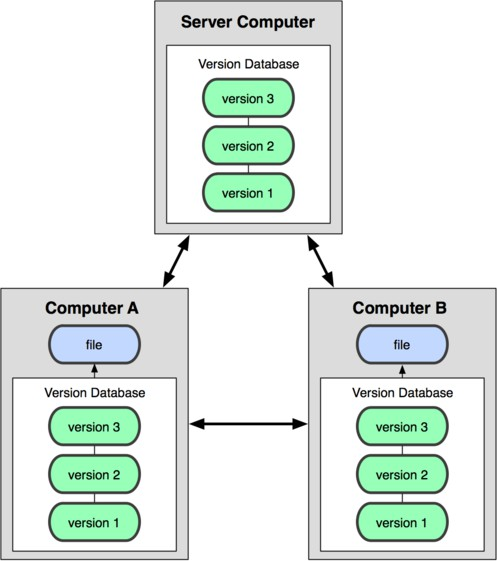
\includegraphics[width=\linewidth]{distributed-vcs.jpeg}
    \end{column}
  \end{columns}
\end{frame}

% =====================================================================
%  19  Git
% =====================================================================
\section{Git}
\dividerslide{Git}

% =====================================================================
%  20  Git snapshots
% =====================================================================
\begin{frame}{Git snapshots}
  \begin{columns}[T]
    \begin{column}{0.4\textwidth}
      \small
      \begin{itemize}
        \item Centralized VCS like Subversion track version data on each \hl{individual file}.
        \item Git keeps ``snapshots'' of the \hl{entire state} of the project.
          \begin{itemize}
            \item Each check-in version of the overall code has a copy of each file in it.
            \item Some files change on a given check-in, some do not.
            \item More redundancy, but faster.
          \end{itemize}
      \end{itemize}
    \end{column}
    \begin{column}{0.58\textwidth}
      \centering
      {\scriptsize\bfseries Subversion}\\[0.5mm]
      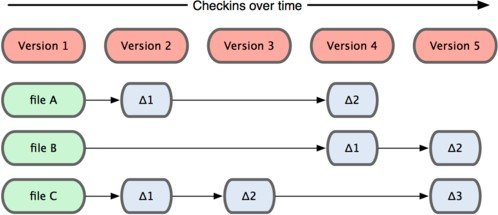
\includegraphics[width=0.72\linewidth]{snapshots-subversion.jpeg}\\[3mm]
      {\scriptsize\bfseries Git}\\[0.5mm]
      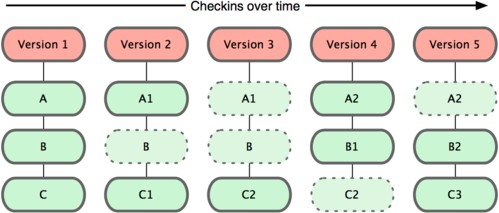
\includegraphics[width=0.72\linewidth]{snapshots-git.jpeg}
    \end{column}
  \end{columns}
\end{frame}

% =====================================================================
%  21  Local git areas
% =====================================================================
\begin{frame}{Local git areas}
  \begin{columns}[T]
    \begin{column}{0.44\textwidth}
      \small
      \begin{itemize}
        \item In your local copy on git, files can be:
          \begin{itemize}
            \item In your local repo
              \begin{itemize}
                \item \hl{committed}
              \end{itemize}
            \item Checked out and modified, but not yet committed
              \begin{itemize}
                \item \hl{working copy}
              \end{itemize}
            \item Or, in-between, in a \hl{``staging'' area}
              \begin{itemize}
                \item ``Staged'' files are ready to be committed.
                \item A commit saves a snapshot of all staged state.
              \end{itemize}
          \end{itemize}
      \end{itemize}
    \end{column}
    \begin{column}{0.54\textwidth}
      \centering
      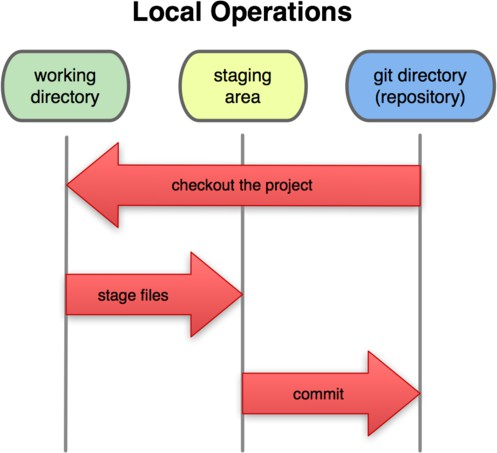
\includegraphics[width=0.78\linewidth]{local-operations.jpeg}\\[1mm]
      {\scriptsize
      \begin{tabular}{p{0.27\linewidth}p{0.2\linewidth}p{0.22\linewidth}}
        \centering Unmodified/ modified Files & \centering Staged Files & \centering\arraybackslash Committed Files
      \end{tabular}}
    \end{column}
  \end{columns}
\end{frame}

% =====================================================================
%  22  Basic Git workflow
% =====================================================================
\begin{frame}{Basic Git workflow}
  \begin{columns}[T]
    \begin{column}{0.46\textwidth}
      \vskip4mm
      \setbeamertemplate{itemize item}{\color{accent}\small$\blacksquare$}
      \begin{itemize}
        \item \textbf{\hl{Modify}} files in your working directory.
        \item \textbf{\hl{Stage}} files, adding snapshots of them to your staging area.
        \item \textbf{\hl{Commit}}, which takes the files in the staging area and stores that
              snapshot permanently to your Git directory.
      \end{itemize}
    \end{column}
    \begin{column}{0.52\textwidth}
      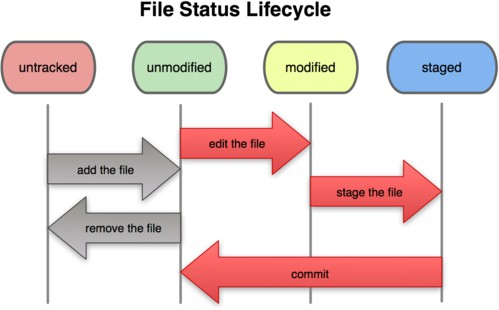
\includegraphics[width=\linewidth]{file-status-lifecycle.jpeg}
    \end{column}
  \end{columns}
\end{frame}

% =====================================================================
%  23  Git commit checksums
% =====================================================================
\begin{frame}{Git commit checksums}
  \small
  \begin{itemize}
    \item In \hl{Subversion} each modification to the central repo increments the version \# of the overall repo.
    \item In \hl{Git}, each user has their own copy of the repo, and commits changes to their local
          copy of the repo before pushing to the central server.
      \begin{itemize}
        \item So Git generates a unique \hl{SHA-1 hash} (40-character hex digits) for every commit, \hl{commit hash}
        \item Refers to commits by this \hl{ID} rather than a version number.
        \item Often we only see the first 7 characters:
          \begin{itemize}
            \item \texttt{1677b2d Edited first line of readme}
            \item \texttt{258efa7 Added line to readme}
            \item \texttt{0e52da7 Initial commit}
          \end{itemize}
      \end{itemize}
  \end{itemize}
\end{frame}

% =====================================================================
%  24  Git Repository
% =====================================================================
\section{Git Repository}
\dividerslide{Git Repository}

% =====================================================================
%  25  Initial Git Configuration
% =====================================================================
\begin{frame}{Initial Git Configuration}
  \vskip2mm
  \begin{itemize}
    \item Set the name and email for Git to use when you commit:
      \begin{itemize}
        \item \cmd{git config --global user.name "Bugs Bunny"}
        \item \cmd{git config --global user.email bugs@gmail.com}
        \item You can call \texttt{git config --list} to verify these are set.
      \end{itemize}
    \vskip2mm
    \item Set the editor that is used for writing commit messages:
      \begin{itemize}
        \item \cmd{git config --global core.editor nano}
          \begin{itemize}
            \item (it is vim editor by default)
          \end{itemize}
      \end{itemize}
  \end{itemize}
\end{frame}

% =====================================================================
%  26  The Repository
% =====================================================================
\begin{frame}{The Repository}
  \small
  \begin{itemize}
    \item Your top-level \hl{working directory} contains everything about your project
      \begin{itemize}
        \item The working directory probably contains many subdirectories---source code,
              binaries, documentation, data files, etc.
        \item One of these subdirectories, named \hl{\texttt{.git}}, is your repository
      \end{itemize}
    \item At any time, you can take a ``snapshot'' of everything (or selected things) in your
          project directory, and put it in your repository
      \begin{itemize}
        \item This ``snapshot'' is called a \hl{commit object}
        \item The commit object contains (1) a set of files, (2) references to the ``parents'' of
              the commit object, and (3) a unique ``SHA1'' name
        \item Commit objects do \emph{not} require huge amounts of memory
      \end{itemize}
    \item You can work as much as you like in your working directory, but the repository isn't
          updated until you \textcolor{bulletblue}{\texttt{commit}} something
  \end{itemize}
\end{frame}

% =====================================================================
%  27  init and the .git repository
% =====================================================================
\begin{frame}{\texttt{init} and the \texttt{.git} repository}
  \vskip3mm
  \begin{itemize}
    \item When you said \cmd{git init} in your project directory, or when you cloned an existing
          project, you create a repository
      \begin{itemize}
        \item The repository is a subdirectory named \cmd{.git} containing various files
        \item The \hl{dot} indicates a ``\hl{hidden}'' directory
        \item You \hl{do} \textcolor{red!75!black}{\emph{not}} \hl{work directly with the contents of}
              \cmd{.git}; various git commands do that for you
      \end{itemize}
  \end{itemize}
\end{frame}

% =====================================================================
%  28  Creating a Git repo
% =====================================================================
\begin{frame}{Creating a Git repo}
  \small
  \begin{itemize}
    \item To create a new \hl{local Git repo} in your current directory:
      \begin{itemize}
        \item \cmd{git init}
          \begin{itemize}
            \item This will create a \texttt{.git} directory in your current directory.
            \item Then you can commit files in that directory into the repo.
          \end{itemize}
        \item \cmd{git add \ph{filename}}
        \item \cmd{git commit -m "\ph{commit message}"}
      \end{itemize}
    \vskip2mm
    \item To \hl{clone a remote repo} to your current directory:
      \begin{itemize}
        \item \cmd{git clone \ph{url localDirectoryName}}
          \begin{itemize}
            \item This will create the given local directory, containing a working copy of the
                  files from the repo, and a \texttt{.git} directory (used to hold the staging
                  area and your actual local repo)
          \end{itemize}
      \end{itemize}
  \end{itemize}
\end{frame}

% =====================================================================
%  29  Git commands
% =====================================================================
\begin{frame}{Git commands}
  \vskip2mm
  \centering\footnotesize
  \renewcommand{\arraystretch}{1.12}
  \begin{tabular}{|l|p{0.5\textwidth}|}
    \hline
    \textbf{command} & \textbf{description}\\ \hline
    \texttt{git clone \ph{url} [\ph{dir}]} & copy a Git repository so you can add to it\\ \hline
    \texttt{git add \ph{file}}             & adds file contents to the staging area\\ \hline
    \texttt{git commit}                     & records a snapshot of the staging area\\ \hline
    \texttt{git status}                     & view the status of your files in the working directory and staging area\\ \hline
    \texttt{git diff}                       & shows diff of what is staged and what is modified but unstaged\\ \hline
    \texttt{git help [\ph{command}]}       & get help info about a particular command\\ \hline
    \texttt{git pull}                       & fetch from a remote repo and try to merge into the current branch\\ \hline
    \texttt{git push}                       & push your new branches and data to a remote repository\\ \hline
    \multicolumn{2}{|c|}{others: \texttt{init, reset, branch, checkout, merge, log, tag}}\\ \hline
  \end{tabular}
\end{frame}

% =====================================================================
%  30  Local Git Repository
% =====================================================================
\section{Local Git Repository}
\dividerslide{Local Git Repository}

% =====================================================================
%  31  Add and commit a file
% =====================================================================
\begin{frame}{Add and commit a file}
  \small
  \begin{itemize}
    \item The first time we ask a file to be tracked, and every time before we commit a file,
          we must add it to the staging area:
      \begin{itemize}
        \item \cmd{git add} \texttt{Hello.java Goodbye.java}
          \begin{itemize}
            \item Takes a snapshot of these files, adds them to the staging area.
            \item In older VCS, ``add'' means ``start tracking this file.'' In Git, ``add'' means
                  ``add to staging area'' so it will be part of the next commit.
          \end{itemize}
      \end{itemize}
    \item To move staged changes into the repo, we commit:
      \begin{itemize}
        \item \cmd{git commit} \texttt{-m "Fixing bug \#22"}
      \end{itemize}
    \item To undo changes on a file before you have committed it:
      \begin{itemize}
        \item \cmd{git reset} \texttt{HEAD -- \ph{filename}}\quad (Unstages the file)
        \item \cmd{git checkout} \texttt{-- \ph{filename}}\quad (Undoes your changes)
      \end{itemize}
    \item[--] All these commands are acting on your local version of repo.
  \end{itemize}
\end{frame}

% =====================================================================
%  32  Making Commits
% =====================================================================
\begin{frame}{Making Commits}
  \small
  \begin{itemize}
    \item You do your work in your project directory, as usual
    \item If you create new files and/or folders, they are \emph{not tracked} by Git unless you ask it to do so
      \begin{itemize}
        \item \cmd{git add} \texttt{\ph{newFile1 newFolder1 newFolder2 newFile2}}
      \end{itemize}
    \item Committing makes a ``snapshot'' of everything being tracked into your repository
      \begin{itemize}
        \item A message telling what you have done is required
        \item \cmd{git commit} \texttt{-m "Uncrevulated the conundrum bar"}
        \item \cmd{git commit}
          \begin{itemize}
            \item This version opens an editor for you to enter the message
            \item To finish, save and quit the editor
          \end{itemize}
      \end{itemize}
    \item Format of the commit message
      \begin{itemize}
        \item One line containing the complete summary
        \item If more than one line, the second line must be blank
      \end{itemize}
  \end{itemize}
\end{frame}

% =====================================================================
%  33  Commits and graphs
% =====================================================================
\begin{frame}{Commits and graphs}
  \small
  \begin{itemize}
    \item A \hl{commit} is when you tell git that a change (or addition) you have made is ready
          to be included in the project
    \item When you commit your change to git, it creates a \hl{commit object}
      \begin{itemize}
        \item A commit object represents the complete state of the project, including all the
              files in the project
        \item The \emph{very first} commit object has no ``parents''
        \item Usually, you take some commit object, make some changes, and create a new commit
              object; the original commit object is the parent of the new commit object
          \begin{itemize}
            \item Hence, most commit objects have a single parent
          \end{itemize}
        \item You can also \hl{merge} two commit objects to form a new one
          \begin{itemize}
            \item The new commit object has two parents
          \end{itemize}
      \end{itemize}
    \item Hence, commit objects form a \hl{directed acyclic graph (DAG)}
      \begin{itemize}
        \item Git is all about using and manipulating this graph
      \end{itemize}
  \end{itemize}
\end{frame}

% =====================================================================
%  34  Commit messages
% =====================================================================
\begin{frame}{Commit messages}
  \vskip3mm
  \begin{itemize}
    \item In git, ``commits are cheap.'' Do them often.
    \item When you commit, you must provide a one-line message communicating what you have
          done (to team members or your future self):
      \begin{itemize}
        \item Terrible message: ``Fixed a bunch of things''
        \item Better message: ``Corrected the calculation of median scores''
      \end{itemize}
    \item You can't say much in one line, so commit often
  \end{itemize}
\end{frame}

% =====================================================================
%  35  Typical workflow
% =====================================================================
\begin{frame}{Typical workflow}
  \begin{columns}[T]
    \begin{column}{0.46\textwidth}
      \vskip4mm
      \begin{itemize}
        \item \cmd{git status}
          \begin{itemize}
            \item See what Git thinks is going on
            \item Use this frequently!
          \end{itemize}
        \item Work on your files
        \item \cmd{git add} \texttt{\textcolor{bulletblue}{yourEditedFiles}}
        \item \cmd{git commit} \texttt{\textcolor{bulletblue}{-m "\emph{What did}"}}
      \end{itemize}
    \end{column}
    \begin{column}{0.52\textwidth}
      \vskip8mm
      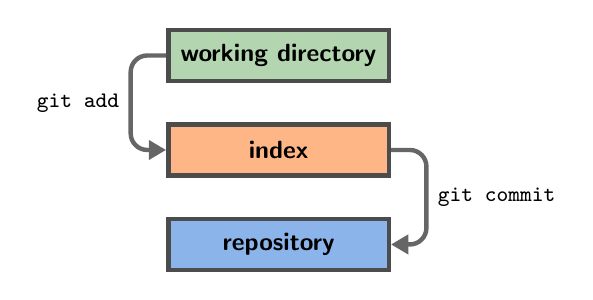
\begin{tikzpicture}[
          box/.style={draw=gray!60!black,line width=1.6pt,minimum width=2.8cm,
                      minimum height=0.65cm,font=\sffamily\bfseries\small},
          flow/.style={-{Triangle[length=2.2mm,width=2.4mm]},gray!80!black,line width=1.6pt,rounded corners=6pt}]
        \node[box,fill=wdgreen]   (wd)   at (0,0)    {working directory};
        \node[box,fill=idxorange] (idx)  at (0,-1.2) {index};
        \node[box,fill=repoblue]  (repo) at (0,-2.4) {repository};
        \draw[flow] (wd.west)  -- ++(-0.45,0) |- node[pos=0.25,left,font=\ttfamily\footnotesize,text=black]{git add} (idx.west);
        \draw[flow] (idx.east) -- ++(0.45,0)  |- node[pos=0.25,right,font=\ttfamily\footnotesize,text=black]{git commit} (repo.east);
      \end{tikzpicture}
    \end{column}
  \end{columns}
\end{frame}

% =====================================================================
%  36  Viewing/undoing changes
% =====================================================================
\begin{frame}{Viewing/undoing changes}
  \small
  \begin{itemize}
    \item To view status of files in working directory and staging area:
      \begin{itemize}
        \item \cmd{git status} or
        \item \cmd{git status -s} (short version)
      \end{itemize}
    \item To see what is modified but unstaged:
      \begin{itemize}
        \item \cmd{git diff}
      \end{itemize}
    \item To see a list of staged changes:
      \begin{itemize}
        \item \cmd{git diff --cached}
      \end{itemize}
    \item To see a log of all changes in your local repo:
      \begin{itemize}
        \item \cmd{git log} or \cmd{git log --oneline} (shorter version)
          \begin{itemize}
            \item \texttt{1677b2d Edited first line of readme}
            \item \texttt{258efa7 Added line to readme}
            \item \texttt{0e52da7 Initial commit}
          \end{itemize}
        \item \cmd{git log -5} (to show only the 5 most recent updates), etc.
      \end{itemize}
  \end{itemize}
\end{frame}

% =====================================================================
%  37  An example workflow
% =====================================================================
\begin{frame}[fragile]{An example workflow}
  \lstset{basicstyle=\ttfamily\footnotesize,escapechar=|,aboveskip=2pt}
  \begin{columns}[T]
    \begin{column}{0.42\textwidth}
\begin{lstlisting}
$ |\textbf{git init}|
$ |\textbf{vi sample.txt}|
$ |\textbf{git status}|
$ |\textbf{git status -s}|
    |\textcolor{red!80!black}{??}| sample.txt
$ |\textbf{git add sample.txt}|
$ |\textbf{git status -s}|
    |\textcolor{green!55!black}{A}|  sample.txt
\end{lstlisting}
    \end{column}
    \begin{column}{0.54\textwidth}
\begin{lstlisting}
|\textit{(update sample.txt in editor)}|
$ |\textbf{git diff}|
|\textbf{diff --git a/sample.txt b/sample.txt}|
|\textbf{index 6231f5a..3e32a85 100644}|
|\textbf{--- a/sample.txt}|
|\textbf{+++ b/sample.txt}|
|\textcolor{cyan!60!black}{@@ -1,3 +1,3 @@}|
 12345
 67890
|\textcolor{red!80!black}{-}|
|\textcolor{green!55!black}{+abcde}|
$ |\textbf{git status -s}|
|\textcolor{green!55!black}{A}\textcolor{red!80!black}{M}| sample.txt
$ |\textbf{git log}|
\end{lstlisting}
    \end{column}
  \end{columns}
\end{frame}

% =====================================================================
%  38  Using GitHub with Eclipse
% =====================================================================
\begin{frame}{Using GitHub with Eclipse}
  \small
  \setbeamertemplate{itemize item}{\color{black}\tiny\textbullet}
  \setbeamertemplate{itemize subitem}{\color{black}\tiny\textbullet}
  \begin{itemize}
    \item Open an account on GitHub
    \item And also create a new repository.
    \item Also create a token (\link{https://github.com/settings/tokens}). You will use this
          token to access your repository on GitHub.
    \item On the Eclipse side:
      \begin{itemize}
        \item Click on your project (in Package Explorer)
        \item On the menu choose \emph{Team -> Share Project}
        \item[] which creates a \emph{local} git repository for you.
      \end{itemize}
    \item Then, again from the menu \emph{Team -> Commit}
    \item Click on the ++ icon to commit staged files (also enter a commit message)
    \item As the third and final step, ``push'' committed changes to the repository you created
          in GitHub account.
  \end{itemize}
\end{frame}

% =====================================================================
%  39  Branch in Git
% =====================================================================
\section{Branch in Git}
\dividerslide{Branch in Git}

% =====================================================================
%  40  What is a Branch in Git?
% =====================================================================
\begin{frame}{What is a Branch in Git\textbf{?}}
  \setbeamertemplate{itemize item}{\color{black}\small\textbullet}
  \vskip2mm
  \begin{itemize}
    \item Branch in Git is a way to keep developing and coding a new feature or modification to
          the software and still not affecting the main part of the project.
  \end{itemize}
  \vskip2mm
  \centering
  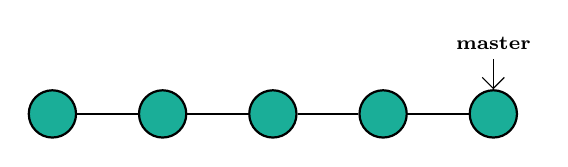
\begin{tikzpicture}[x=1.4cm]
    \foreach \i in {0,...,4} \node[cmain] (n\i) at (\i,0) {};
    \foreach \i [evaluate=\i as \j using int(\i+1)] in {0,...,3} \draw[thick] (n\i) -- (n\j);
    \node[ref] (m) at (4,0.9) {master};
    \draw[refarr] (m) -- (n4);
  \end{tikzpicture}
  \vskip2mm
  \raggedright
  \begin{itemize}
    \item \textbf{\emph{The primary or default branch in Git is the master branch (similar to a
          trunk of the tree)}}. As soon as the repository creates, so does the master branch
          (\emph{or the default branch}).
  \end{itemize}
\end{frame}

% =====================================================================
%  41  Branching in Git (1)
% =====================================================================
\begin{frame}{Branching in Git}
  \setbeamertemplate{itemize item}{\color{black}\small\textbullet}
  \begin{itemize}
    \item You have been working on a project with the client being happy until this point.
  \end{itemize}
  \centering
  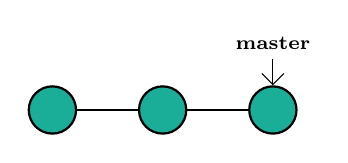
\begin{tikzpicture}[x=1.4cm]
    \foreach \i in {0,1,2} \node[cmain] (n\i) at (\i,0) {};
    \draw[thick] (n0) -- (n1) -- (n2);
    \node[ref] (m) at (2,0.85) {master};
    \draw[refarr] (m) -- (n2);
  \end{tikzpicture}
  \raggedright
  \begin{itemize}
    \item After that, you decide to develop a feature and create a new branch called feature for
          the same purpose and start working on it.
  \end{itemize}
  \centering
  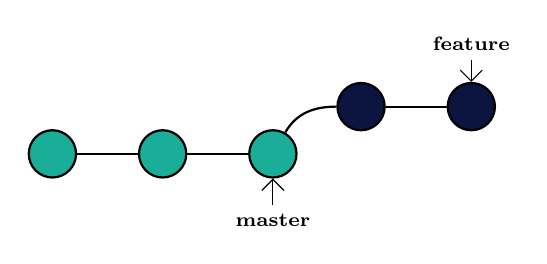
\begin{tikzpicture}[x=1.4cm]
    \foreach \i in {0,1,2} \node[cmain] (n\i) at (\i,0) {};
    \node[cfeat] (f1) at (2.8,0.6) {};
    \node[cfeat] (f2) at (3.8,0.6) {};
    \draw[thick] (n0) -- (n1) -- (n2);
    \draw[thick] (n2) to[out=60,in=180] (f1);
    \draw[thick] (f1) -- (f2);
    \node[ref] (fr) at (3.8,1.4) {feature};
    \draw[refarr] (fr) -- (f2);
    \node[ref] (m) at (2,-0.85) {master};
    \draw[refarr] (m) -- (n2);
  \end{tikzpicture}
\end{frame}

% =====================================================================
%  42  Branching in Git (2)
% =====================================================================
\begin{frame}{Branching in Git}
  \setbeamertemplate{itemize item}{\color{black}\small\textbullet}
  \begin{columns}[T]
    \begin{column}{0.47\textwidth}
      \small
      \begin{itemize}
        \item In the meantime, you decide to develop another feature and wait for the client's approval.
      \end{itemize}
      \vskip2mm
      \centering
      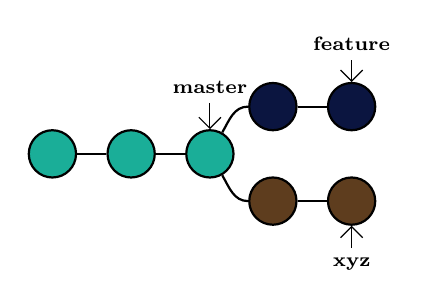
\begin{tikzpicture}[x=1.0cm]
        \foreach \i in {0,1,2} \node[cmain] (n\i) at (\i,0) {};
        \node[cfeat] (f1) at (2.8,0.6)  {};
        \node[cfeat] (f2) at (3.8,0.6)  {};
        \node[cxyz] (x1) at (2.8,-0.6) {};
        \node[cxyz] (x2) at (3.8,-0.6) {};
        \draw[thick] (n0) -- (n1) -- (n2);
        \draw[thick] (n2) to[out=60,in=180] (f1);  \draw[thick] (f1) -- (f2);
        \draw[thick] (n2) to[out=-60,in=180] (x1); \draw[thick] (x1) -- (x2);
        \node[ref] (fr) at (3.8,1.4) {feature}; \draw[refarr] (fr) -- (f2);
        \node[ref] (m)  at (2,0.85)  {master};  \draw[refarr] (m) -- (n2);
        \node[ref] (xr) at (3.8,-1.4) {xyz};    \draw[refarr] (xr) -- (x2);
      \end{tikzpicture}
    \end{column}
    \begin{column}{0.5\textwidth}
      \small
      \begin{itemize}
        \item Now, since you were following the branched strategy, you need to remove the
              branch, and all the remaining code remains as it is.
        \item The new feature can be easily added to the master branch to achieve the following.
      \end{itemize}
      \vskip0mm
      \centering
      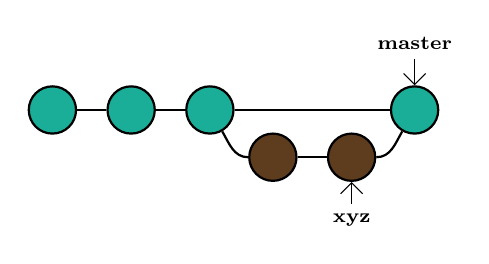
\begin{tikzpicture}[x=1.0cm]
        \foreach \i in {0,1,2} \node[cmain] (n\i) at (\i,0) {};
        \node[cxyz] (x1) at (2.8,-0.6) {};
        \node[cxyz] (x2) at (3.8,-0.6) {};
        \node[cmain] (n3) at (4.6,0) {};
        \draw[thick] (n0) -- (n1) -- (n2) -- (n3);
        \draw[thick] (n2) to[out=-60,in=180] (x1); \draw[thick] (x1) -- (x2);
        \draw[thick] (x2) to[out=0,in=-120] (n3);
        \node[ref] (m)  at (4.6,0.85) {master}; \draw[refarr] (m) -- (n3);
        \node[ref] (xr) at (3.8,-1.4) {xyz};    \draw[refarr] (xr) -- (x2);
      \end{tikzpicture}
    \end{column}
  \end{columns}
\end{frame}

% =====================================================================
%  43  Branching and Merging
% =====================================================================
\begin{frame}{Branching and Merging}
  \setbeamertemplate{itemize item}{\color{black}\small\textbullet}
  \setbeamertemplate{itemize subitem}{\color{accent}--}
  \small
  \hspace*{3mm}Git uses branching heavily to switch between multiple tasks.
  \begin{itemize}
    \item To create a new local branch:
      \begin{itemize}\item \cmd{git branch \ph{name}}\end{itemize}
    \item To list all local branches: (* = current branch)
      \begin{itemize}\item \cmd{git branch}\end{itemize}
    \item To switch to a given local branch:
      \begin{itemize}\item \cmd{git checkout \ph{branchname}}\end{itemize}
    \item To merge changes from a branch into the local master:
      \begin{itemize}
        \item \cmd{git checkout master}
        \item \cmd{git merge \ph{branchname}}
      \end{itemize}
  \end{itemize}
\end{frame}

% =====================================================================
%  44  Resources
% =====================================================================
\section{Resources}
\dividerslide{Resources}

% =====================================================================
%  45  Installing/learning Git
% =====================================================================
\begin{frame}{Installing/learning Git}
  \vskip3mm
  \begin{itemize}
    \item Git website: \link{http://git-scm.com/}
      \begin{itemize}
        \item Free on-line book: \link{http://git-scm.com/book}
        \item Git for Computer Scientists:
          \begin{itemize}
            \item \link{http://eagain.net/articles/git-for-computer-scientists/}
          \end{itemize}
      \end{itemize}
    \vskip2mm
    \item At command line: (where verb = config, add, commit, etc.)
      \begin{itemize}
        \item \cmd{git help \ph{verb}}
      \end{itemize}
  \end{itemize}
\end{frame}

\end{document}
